\section{Exp6: Pose estimation from camera}

Using the LIDAR for pose estimation of the cube required that no other objects
were accidentally measured, and used the fact that the position of the cube can
be described by two lines in the plane. A more general approach is to infer the
pose from a camera. A usual setup in robotics is to have a camera at a fixed
position and infer poses under the assumption that the camera does not shift
position. Experiments are here first described for estimation under this
assumption and then extended for estimation from a non-fixed camera.

\subsection{Pose estimation from fixed camera}

A camera was mounted at a fixed position as shown in figure
\ref{fig:camera_placement_fixed}. LIDAR was used to label the pose of the cube
in the coordinate frame of the robot.  In total, 10'000 RGB images were
collected during execution of the trained policy. For each picture, a depth
channel was also collected to evaluate the difference in performance when
adding this information. For the depth channel, the camera returns numbers in
the range $[0, 255]$ aligned for each pixel in the color image. The distance
$0$ is in practice never registered but used to represent that depth for this
pixel is missing.

\begin{figure}[h!]
    \centering
    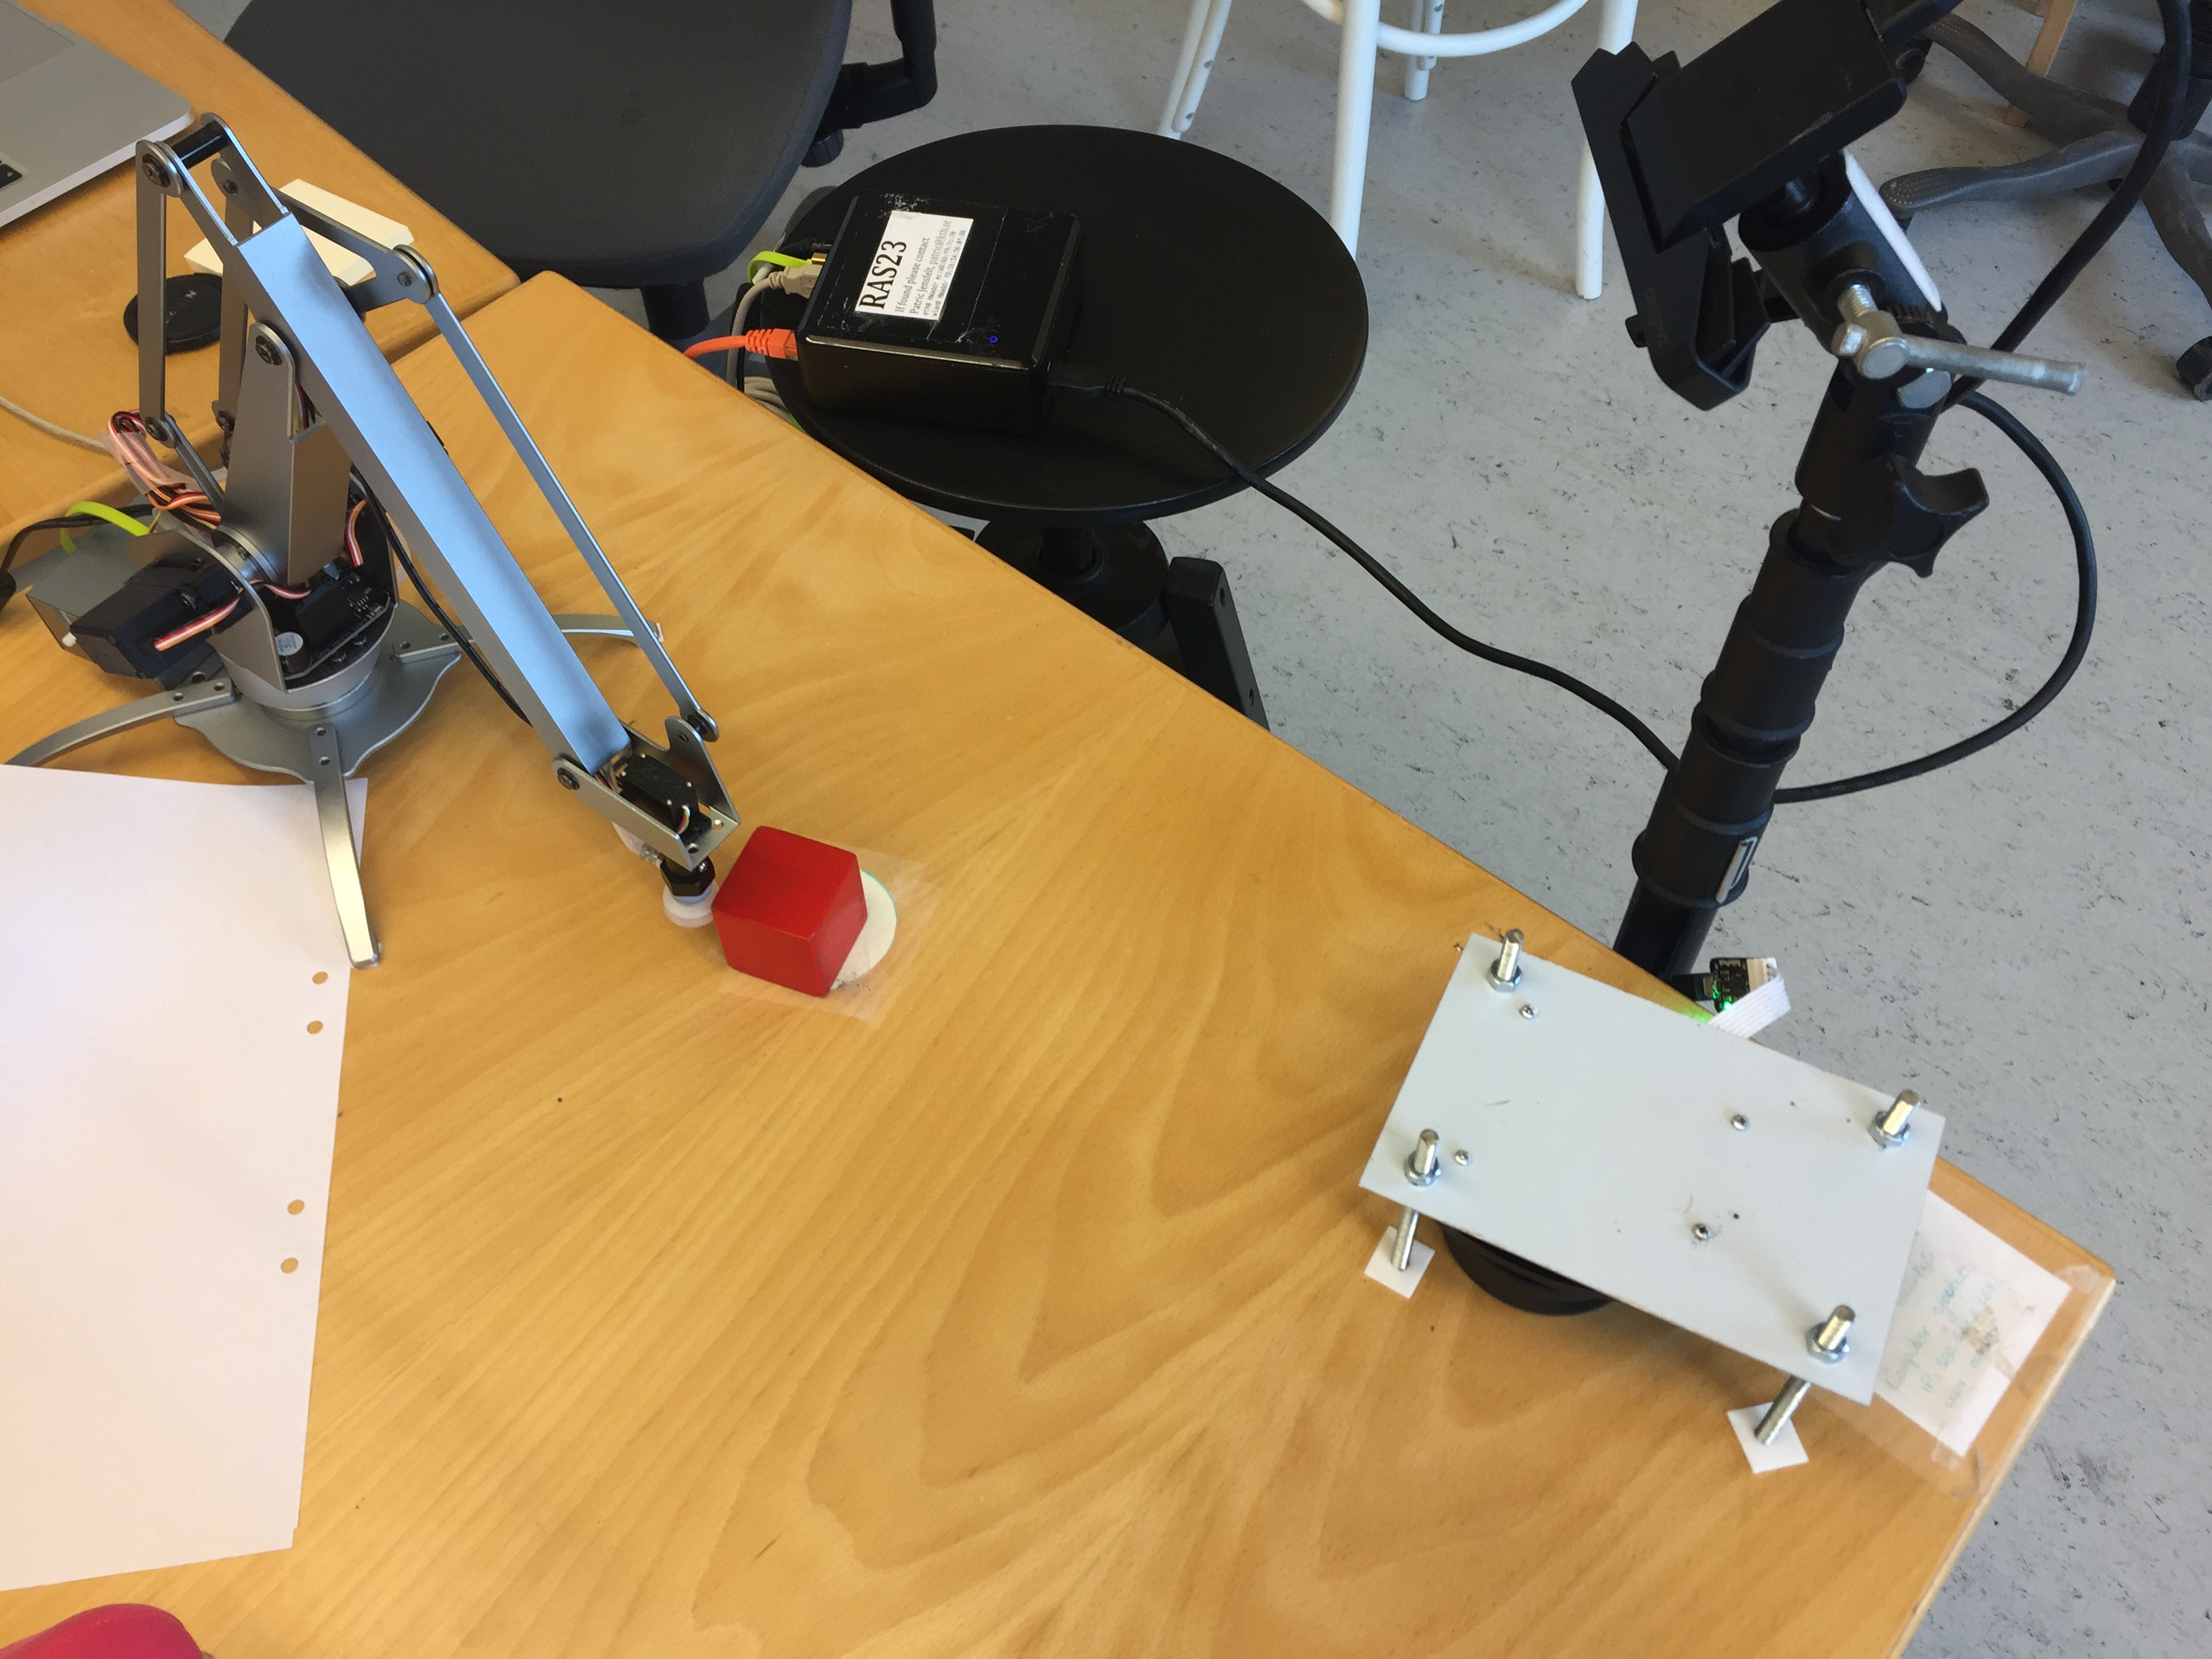
\includegraphics[width=0.4 \textwidth]{res/camera_placement_fixed.jpg}

    \caption{Fixed camera placement for pose estimation of the cube.}

    \label{fig:camera_placement_fixed}
    
\end{figure}

The first part of the network in figure \ref{fig:gps_net} was used, with two
hidden layers of 100 hidden ELU activated units each after the 2-D expected
position. The output was a 2-dimensional linear layer predicting the cube
position in the robot coordinate frame. For incorporating depth into the
network, I propose a layout, shown in figure \ref{fig:depth_net}, where depth
is input at two locations in the network. The first place is simply as a fourth
dimension into the first convolutional layer. The second place is to append the
expected distance $\mathbb{E}[D_k]$ for each feature $k \in [1, 32]$ to the
fully connected layers, using the spatial softmax as the probability when
calculating the expectation:

\begin{figure}[h!]
    \centering
    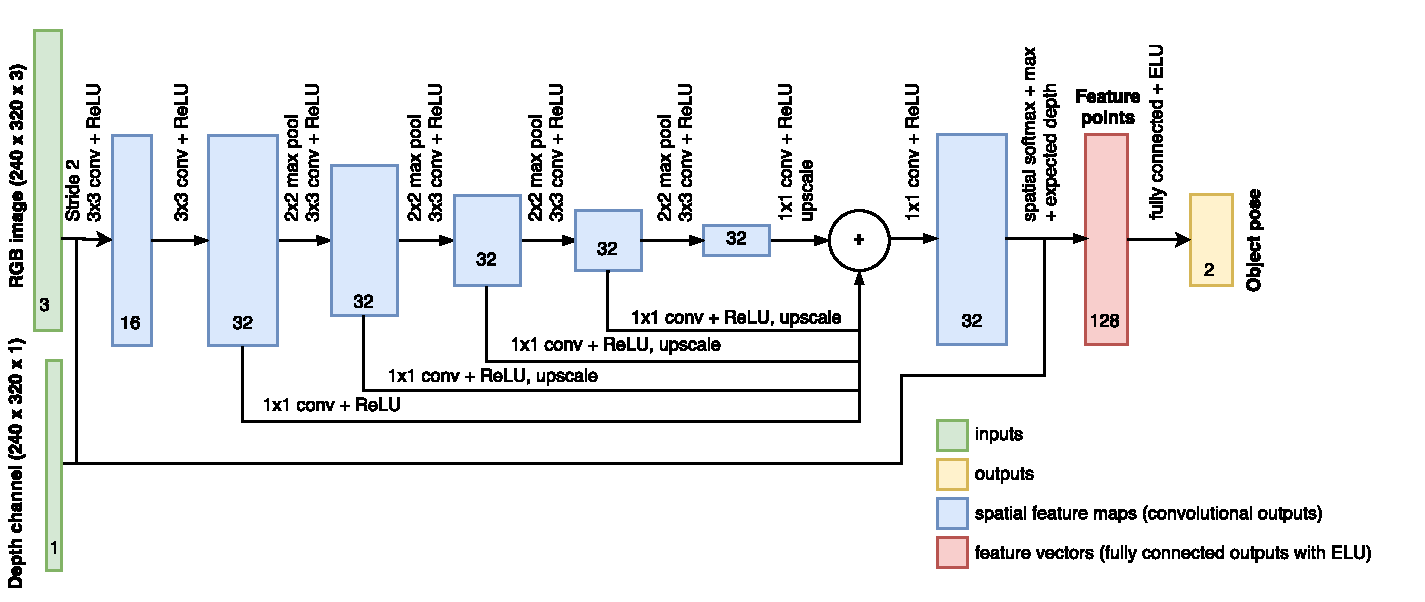
\includegraphics[width=1.0 \textwidth]{res/depth_net.pdf}

    \caption{Proposed pose estimation network incorporating depth information.
    Input to the first convolutional layer is a 4-channel RGBD image.  Using
    the spatial softmax as a per-feature probability distribution, expected
    depths per feature map are also concatenated with the expectation over
    image coordinates. As a measure of uncertainty in each feature, the maximum
    activation for each feature map, after the spatial softmax, are also
    concatenated with the input to the fully connected layer.}

    \label{fig:depth_net}
    
\end{figure}

\begin{equation}
    \mathbb{E}[D_{k}] = \sum_{i, j} p(c_{i, j, k}) d_{i, j}
\end{equation}

Here, $p(c_{i, j, k})$ is the output of the spatial softmax at pixel $(i, j)$
for feature map $k$ and $d_{i, j}$ the registered depth at pixel $(i, j)$. The
network was trained by minimizing the mean square error and using the Adam
optimizer. The training and validation losses are plotted in figure
\ref{fig:depth-vs-rgb} showing that only using RGB converges faster and that
adding depth did not contribute to better scores in this experiment.

\begin{figure}[h!]
    \centering
    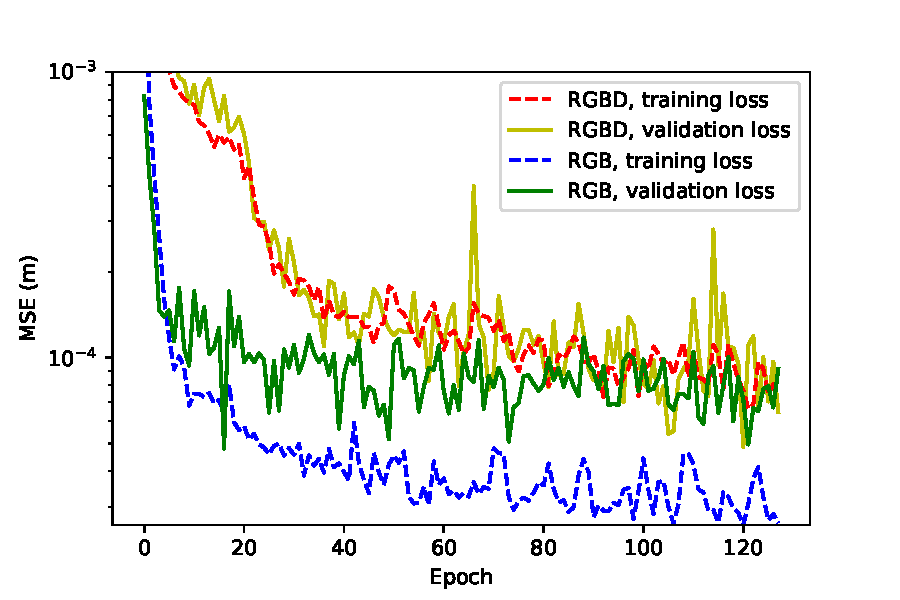
\includegraphics[width=0.6 \textwidth]{res/depth-vs-rgb.pdf}

    \caption{Training curves for pose estimation from a fixed position camera.
    Adding depth information did not lower training scores, only slowing down
    the time needed to converge.}

    \label{fig:depth-vs-rgb}
    
\end{figure}

The trained network using RGB was used instead of the pose estimates from the
LIDAR and tested on a robot. The network needed significantly more time to
evaluate than when using the LIDAR estimates. A video was recorded of the
result and can be seen here: \url{https://youtu.be/vakM-xvhEmE}. A dark gray
cup was added into the workspace without previous tests during recording of the
video showing that the estimation could handle some distraction. Further tests
showed that any red object will disturb the pose estimates, making the policy
unsuccessful in pushing the cube. This was expected though since no distractors
were added during data collection.

\subsection{Simulating a movable camera}
\label{subsec:sim_moving}

In order to estimate the pose of some object in some coordinate frame, the
offset of the camera with respect to this frame must be known, or that some
feature in the input data defines this coordinate frame. Since the region
around the end-effector in these experiments is non-symmetric (see left part of
figure \ref{fig:end-effector-frame}), this area could be used to define a
coordinate frame as long as this part is visible to the camera. Let this
coordinate frame be defined as in the right side of figure
\ref{fig:end-effector-frame}.

\begin{figure}[h!]
    \centering
    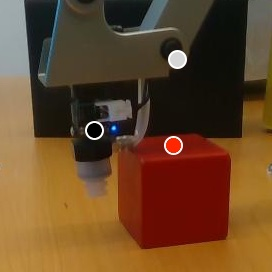
\includegraphics[width=0.32 \textwidth]{res/pose-feature-points.jpg}
    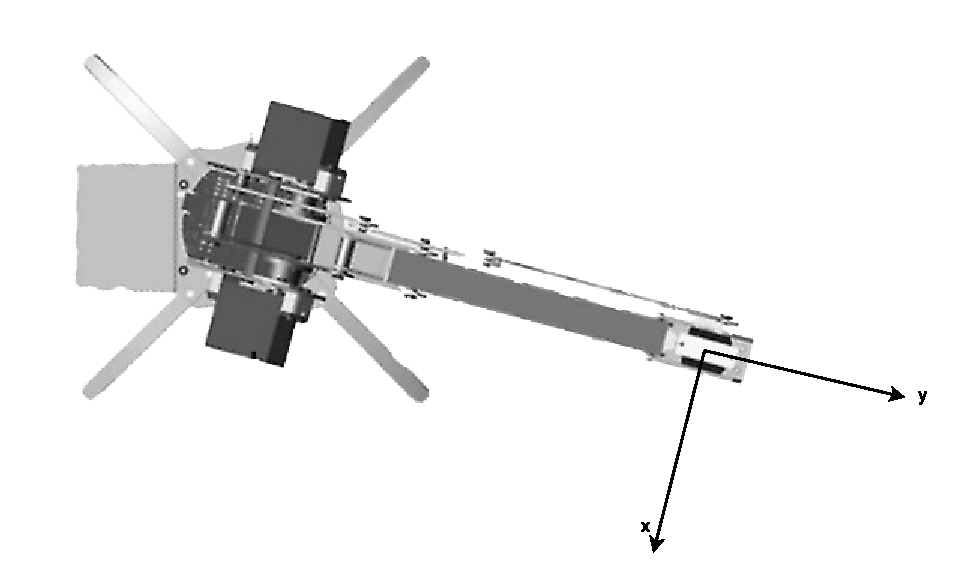
\includegraphics[width=0.5 \textwidth]{res/end-effector-frame.pdf}

    \caption{If the section of the robot to the left is visible, it can define
    a coordinate frame for the cube invariant to camera rotation and
    translation.}

    \label{fig:end-effector-frame}
    
\end{figure}

Simulated experiments were first done in order to investigate whether relative
poses of two objects can be inferred from 2-d projections of those 3-d points.
Inspired by the three marked points in figure \ref{fig:end-effector-frame}, an
environment was setup where these points together with different camera
positions and orientations could be sampled and projected onto a 2-d plane (the
image). Some samples are shown in figure \ref{fig:pose-sim-setup}. The target
values were given in the frame of the end effector; a 2-d horizontal coordinate
frame with the origin at the suction cup and x-, and y-axes parallel to the
table.

\begin{figure}[h!]
    \centering
    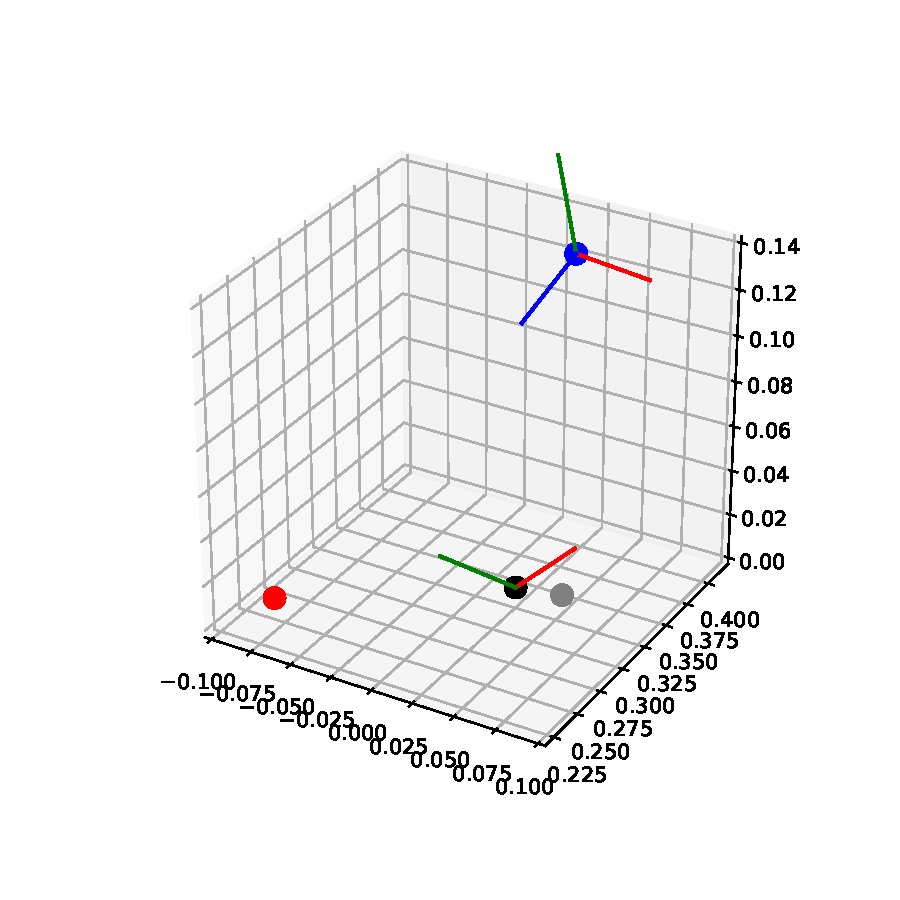
\includegraphics[width=0.32 \textwidth]{res/pose_sim_setup1.pdf}
    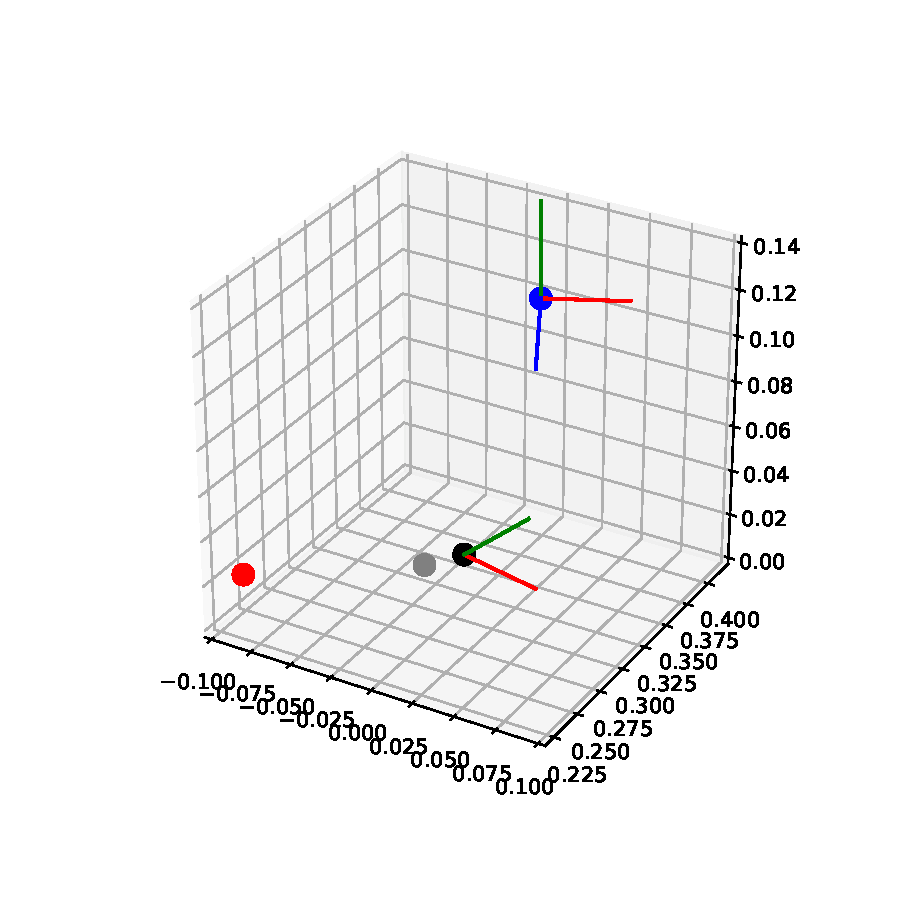
\includegraphics[width=0.32 \textwidth]{res/pose_sim_setup2.pdf}
    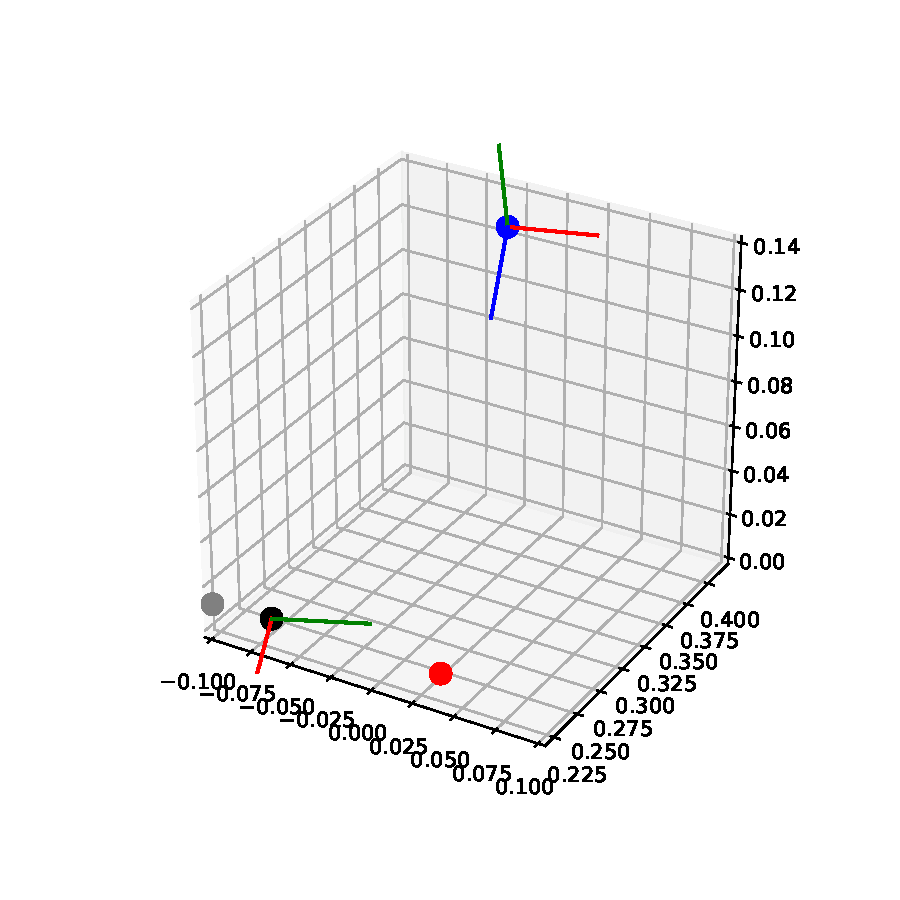
\includegraphics[width=0.32 \textwidth]{res/pose_sim_setup3.pdf}

    \caption{Sampled camera (blue), cube (red), and robot poses (black and
    gray). Target values were cube poses in the frame given by the robot, here
    seen with origin in the black point with x-, and y-axis shown as the red
    and green lines. Input data were the three points projected onto a 2-d
    plane given by the camera and a focal length $f$. Comparisons were made
    when appending a third dimension to the picture, which was the length from
    camera to each point.}

    \label{fig:pose-sim-setup}
    
\end{figure}

All the operations needed to infer the target values from known 3-d coordinates
were linear transformations, giving rise to question if it is sufficient to
regress a linear model. Experiments were therefore done with a linear model,
and a one and two hidden layer model with 100 hidden ELU-activated units and
batch normalization, and including or excluding depth information. The loss was
mean squared error and the networks were trained using the Adam optimizer.
Clearly, as can be seen in figure \ref{fig:pose-sim-losses} and
\ref{fig:pose-sim-corr}, deeper networks achieve better results. 2-d
coordinates were also shown to be sufficient, although depth information
improves the results. Interestingly, the predictions for a 2 hidden layer with
depth information is still quite noisy, even though the 2D feature points are
given without noise. This raises concerns to whether good enough results can be
achieved with real data where feature coordinates are inferred by a
convolutional neural network, and also where labels are produced with noise.

\begin{figure}[h!]
    \centering
    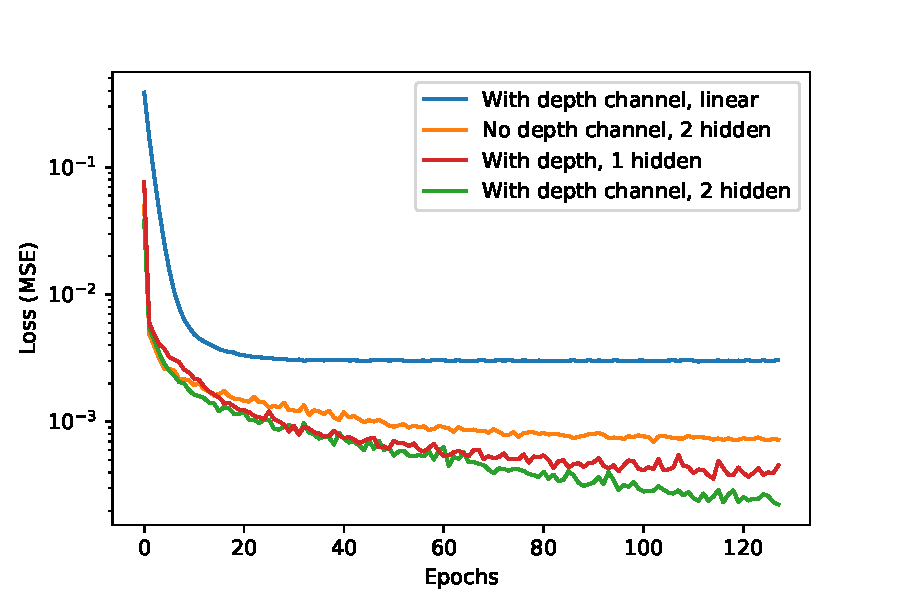
\includegraphics[width=0.7 \textwidth]{res/pose_sim_losses.pdf}

    \caption{Training losses for pose estimation of simulated robot and cube.
    Losses for neural networks given different parametrizations and input
    data.}

    \label{fig:pose-sim-losses}
    
\end{figure}

\begin{figure}[h!]
    \centering
    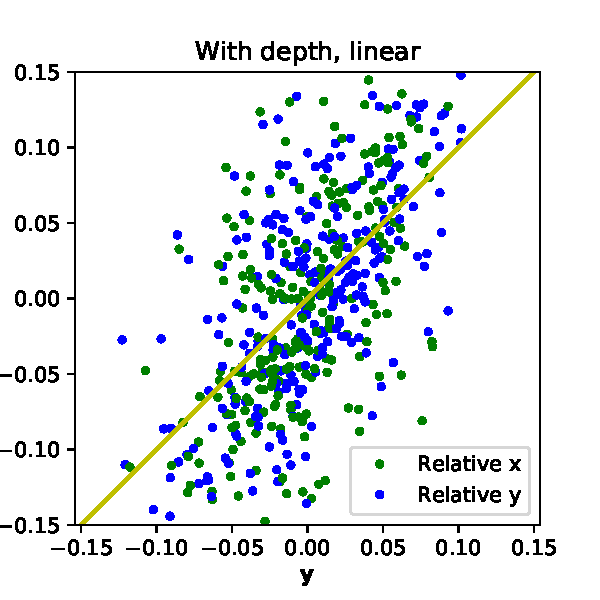
\includegraphics[width=0.2 \textwidth]{res/pose_sim_depth_linear.pdf}
    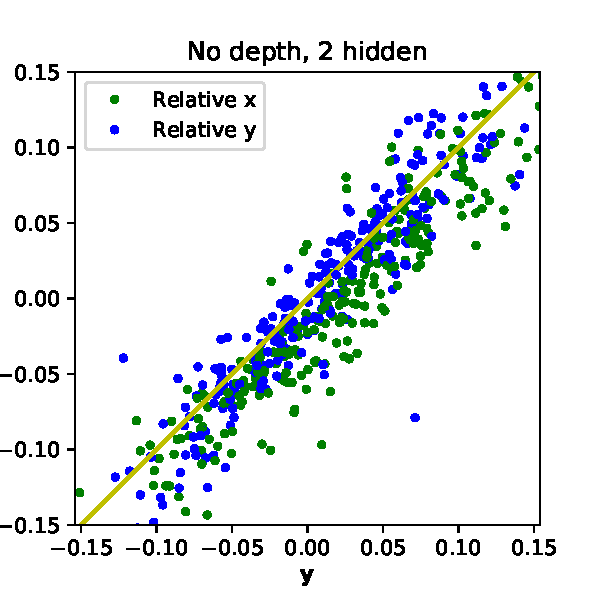
\includegraphics[width=0.2 \textwidth]{res/pose_sim_nodepth_2hidden.pdf}
    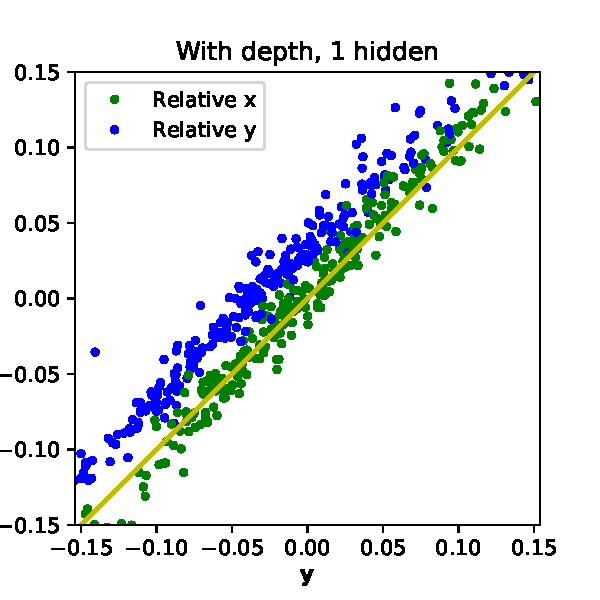
\includegraphics[width=0.2 \textwidth]{res/pose_sim_depth_1hidden.pdf}
    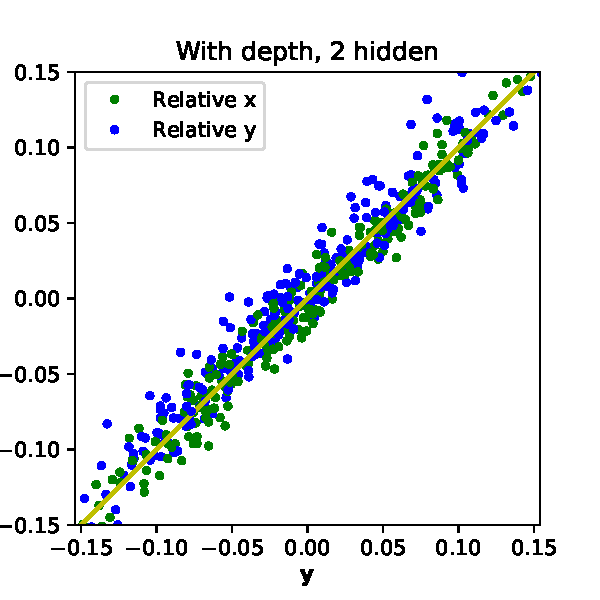
\includegraphics[width=0.2 \textwidth]{res/pose_sim_depth_2hidden.pdf}

    \caption{Pose estimation from a simulated environment and camera. Target
    $x$ (green) and target $y$ (blue) values plotted against the predicted
    $x$ and $y$ values.  Plot 1: Depth information was provided to the two
    points on the robot and the cube. Network was only a linear layer. Plot 2:
    Only 2-d coordinates were given as inputs, network had 2 hidden layers.
    Plot 3: Depth was given, network using 1 hidden layer.  Plot 4: Depth was
    given, network using 2 hidden layers.}

    \label{fig:pose-sim-corr}
    
\end{figure}

\subsection{Movable camera in the real setup}

RGB images were collected while executing the pushing policy on one of the
robots. The images were labeled with relative poses to the end-effector using
the position estimates of the cube using the LiDAR, and the arm using the
forward kinematics on the servo angles. The camera was placed at random
positions around the workspace, always capturing at least the portion of the
arm as shown in figure \ref{fig:end-effector-frame}, and capturing at least the
top surface of the cube. Distracting objects were put into the scene such as
different kinds of rubble in the background, changing the appearance of the
table surface, changing light conditions, and playing up videos in the
background. Some of the training images are shown in figure
\ref{fig:relpose-training-data}. Images were augmented during training by
adding Gaussian noise, randomly scaling and translating the image, and randomly
shifting the color channels. The network in figure \ref{fig:depth_net} was used
with some modifications. As previous results (section \ref{subsec:sim_moving})
showed better performance using 2 fully connected hidden layers with 100 units
each, this was used as last layers, together with batch normalization. Depth
images were also collected and trained on, but showed to be overfitting before
good models were found. Adding regularization in the form of dropout and weight
decay did help against overfitting when using depth, but instead resulted in
worse validation scores.

\begin{figure}[h!]
    \centering
    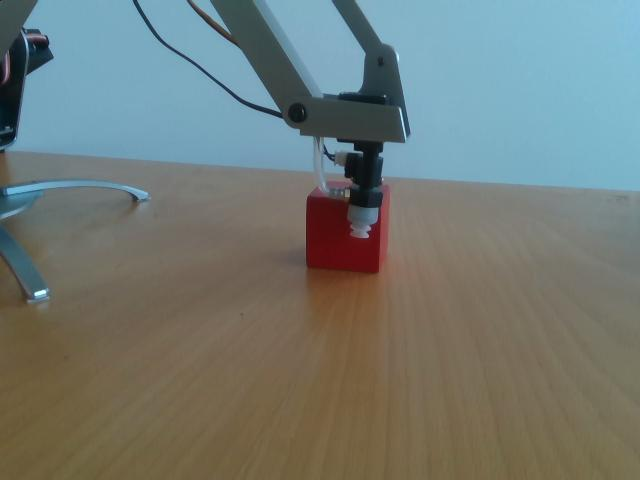
\includegraphics[width=0.3 \textwidth]{res/spiderman1.jpg}
    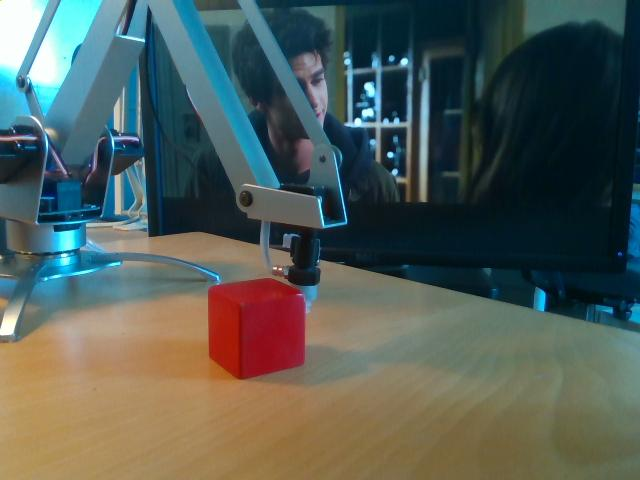
\includegraphics[width=0.3 \textwidth]{res/spiderman2.jpg}
    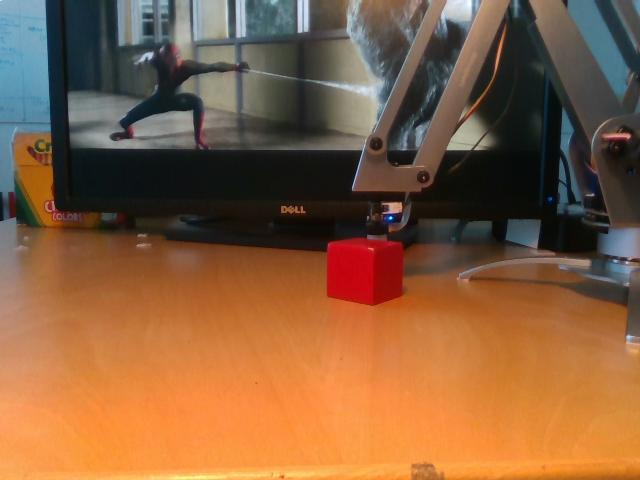
\includegraphics[width=0.3 \textwidth]{res/spiderman3.jpg}

    \caption{Data gathering for pose estimation in coordinate frame defined by
    the position and orientation of the end-effector. Camera was randomly
    placed at different positions, angles, and heights. To make predictions
    robust, images were recorded using different lighting conditions, different
    table surfaces, and different backgrounds.}

    \label{fig:relpose-training-data}
    
\end{figure}

\subsection{Evaluating the trained network for the movable camera}

Plotting the labels against the predicted values show that the network can
learn the relative poses, albeit the precision being roughly $\pm 1$ cm was not
good enough to get robust results on the robots. Plots of labels plotted
against predicted values are shown in figure \ref{fig:relpose_end2end_results}.
Roughly estimating the influence of the resolution gives the following: Assume
the cube is at such a distance that $8$ cubes fit next to each other while all
of them are still fitting inside the image borders. The input image has a width
of $340$ pixels, dividing the total width of $8$ cubes by the $340$ pixels
gives:

\begin{equation}
    4 \cdot 8 \text{ cm / } 340 \text{ pixels } \approx 0.09 \text{ cm / pixel } \approx 1 \text{ mm / pixel }
\end{equation}

The intermediary representation has half the resolution implying approximately
$2$ mm / pixel which can only to a small extent explain the noisy predictions.
On top of this, pose estimates were shown to vary approximately $\pm 5$ mm from
scan to scan, partially explaining the appearance of the plots in figure
\ref{fig:relpose_end2end_results}. The fact remains though that when running
estimation on one of the real robots, it failed to give stable results.

\begin{figure}[h!]
    \centering
    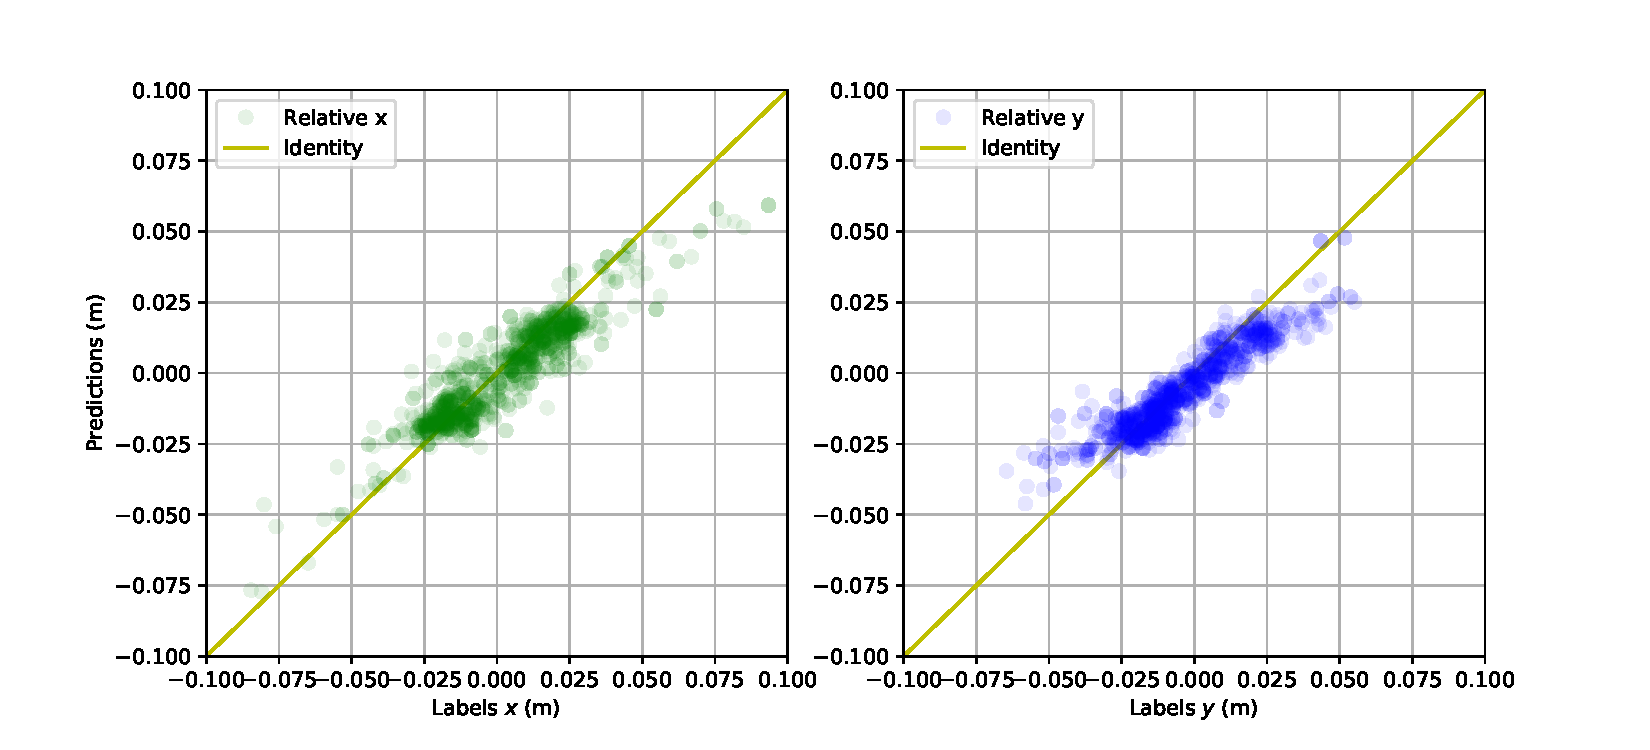
\includegraphics[width=0.8 \textwidth]{res/results_relative_pose_end2end.pdf}

    \caption{Results for estimating the cube pose in the end-effector frame using
    RGB-images from a camera at random positions, heights, and orientations. Target values
    (horizontal axis) are plotted against predicted values (vertical axis). The model
    predictions were too inaccurate to produce good results on the robots for the
    pushing task.}

    \label{fig:relpose_end2end_results}
    
\end{figure}

